\section{Results}\label{sec:results}

In this section, the concrete implementation of the described models in \autoref{sec:methods} and the resulting results are presented. The focus of the elaborations is on the major findings of the work by Tran and Yates; accordingly, not all results are listed herein. Details can be studied in the paper by Tran and Yates \cite{tran2022dense}.

\subsection{Experimental Setup}

Tran and Yates implemented their models in a TensorFlow (Abadi et al. \cite{abadi2016tensorflow}) setup: For the pretrained language model, they chose a distilled BERT (Sanh et al. \cite{sanh2019distilbert}), fine-tuned it using TAS BERT approach (Hofst{\"a}tter et al. \cite{tasbert}), as described in \autoref{subsec:general_model}. To determine the embeddings, they used Dexter (Ceccarelli et al. \cite{ceccarelli2013dexter}) and Wikipedia2Vec (Yamada et. al \cite{yamada2018wikipedia2vec}), as explained in \autoref{subsec:entity_embeddings}. 

Training was conducted using pairwise hinge loss on four Quadro RTX 8000 GPUs in parallel, employing 300,000 training samples from the MS MARCO dataset (Nguyen et al. \cite{nguyen2016ms}). For the models allowing indexing (EVA Single and EVA Multi, see \autoref{subsec:models}), the end-trained model was used to index embeddings for documents. Evaluation was performed on 7,127 test samples from the MS Marco dataset and the datasets TREC Deep Learning (DL) Track 2019 (MacAvaney et al. \cite{trec_dl_2019}), TREC DL 2020 (MacAvaney et al. \cite{trec_dl_2020}), TREC DL HARD (Yates et al. \cite{dl_hard}). Evaluation metrics were chosen to be nDCG@10, MRR@10, MAP@1000.

The models proposed by Tran and Yates (EVA Single, EVA Single-QA, and EVA Multi, as described in \autoref{subsec:models}) were compared against various baselines as BM-25, TAS BERT, ERNIE and others. Details can be examined within the paper by Tran and Yates \cite{tran2022dense}.
\begin{comment}
\begin{itemize}
    \item BM25: The most prominent example of exact matching paradigm, using sparse representations (Robertson et al. \cite{BM25})
    \item TAS BERT: Fine-tuned BERT model using topic-aware sampling strategy as described in \autoref{subsec:general_model}.
    \item ANCE: A state-of-the-art bi-encoder model that employs a sophisticated negative sample mining strategy during training process (Xiong et al. \cite{xiong2020approximate}).
    \item BM25 + T5 (Zero-Shot): First stage ranking using BM25 plus a T5-cross-encoder (Nogueira et al. \cite{nogueira2020document}) to rerank the top 1000 results of first stage retrieval.
    \item ERNIE: Fine-tuned model of ERNIE v2 (Sunh et. al. \cite{sun2020ernie}), which is an optimized version of base ERNIE as described in \autoref{sec:related_work}.
    \item ERNIE Multi: Similar to the EVA Multi approach, but using ERNIE as a pre-trained language model for word embeddings.
    \item Best Reported: The best results of the MS MARCO leader board or respectively the best results of the corresponding papers of the TREC DL datasets (MacAvaney et al. \cite{trec_dl_2019}, MacAvaney et al. \cite{trec_dl_2020}, Yates et al. \cite{dl_hard}).
\end{itemize}
\end{comment}

\subsection{Efficiency}\label{sec:efficiency}

The evaluation of different models by Tran and Yates included both efficiency and effectiveness. Complete results for both aspects can be found in the paper by Tran and Yates \cite{tran2022dense}. In terms of efficiency, particular attention was paid to latency, and the results for all models under examination are presented in \autoref{tab:results_effectiveness}. The table displays the average search time per query across all evaluation datasets for each model, all executed on the same server.

\def\arraystretch{1.2}
\begin{table}[!htb]
    \small
    \centering
    \begin{tabular}{l|l}
    \textbf{Methods}                                        & \textbf{Latency (ms)} \\ \hline
    \textit{\textbf{Low latency (\textless{}100 ms)}}       & \textit{\textbf{}}    \\ \hline
    BM25                                                    & 13                    \\
    ANCE                                                    & 25                    \\
    ERNIE Tuned                                             & 29                    \\
    ERNIE Multi                                             & 70                    \\
    TAS BERT                                                & 28                    \\
    EVA Single                                              & 40                    \\
    EVA Multi                                               & 76                    \\
    EVA Multi-KNRM                                          & 74                    \\ \hline
    \textit{\textbf{Higher latency (\textgreater{}100 ms)}} & \textit{\textbf{}}    \\ \hline
    EVA Single-QA                                           & 2,039                  \\
    EVA Single-QA-KNRM                                      & 3,839                  \\
    BM25 + T5 (Zero-Shot)                                   & 5,052                  \\ \hline
    Best Reported                                           & -                    
    \end{tabular}
    \caption{Analysis of effectiveness of EVA models and baselines}
    \label{tab:results_effectiveness}
\end{table}

\subsection{Effectiveness}\label{sec:effectiveness}

The effectiveness results of the various models consistently hold across all combinations of evaluation metrics and datasets. To avoid redundancy, this report will provide exemplary results based on the nDCG@10 metric and the TREC DL Track 2019 dataset \cite{trec_dl_2019}, which serve as representatives of the overall results. These exemplary results are illustrated in a visual format in \autoref{fig:results}. Further details on the main outcomes can be found in the subsequent \autoref{subsec:outcomes}.

\begin{figure}[!htb]
    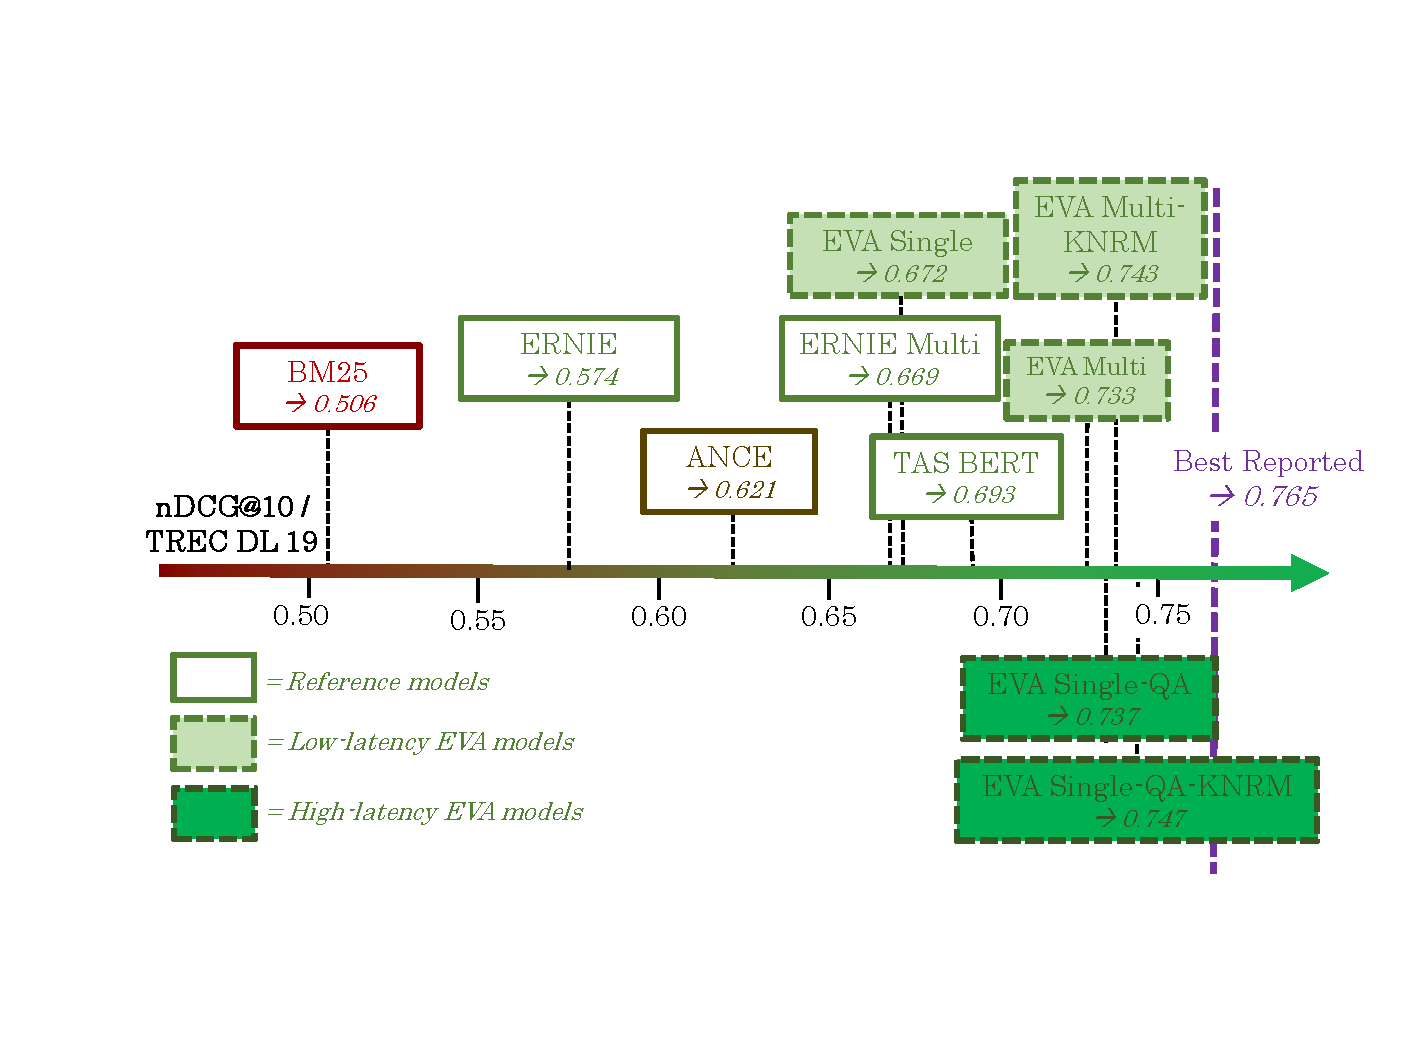
\includegraphics[trim={1.5cm 3cm 0.7cm 3cm}, clip, width=\textwidth]{resources/results} 
    \caption{Exemplary results of EVA models and baselines for TREC DL 19 dataset and evaluation metric nDCG@10}
    \label{fig:results}
\end{figure}

\subsection{Impact}\label{subsec:outcomes}

The outcomes of Tran and Yates' work, based on the results from \autoref{sec:effectiveness} and \autoref{sec:efficiency}, can be summarized as follows:
\begin{enumerate}
    \item \textbf{Enriching pre-trained language models with entity embeddings improve effectiveness significantly}:
    The effectiveness results demonstrate that the models proposed by Tran and Yates, namely EVA Multi and EVA Single-QA, both with and without KNRM signal, outperform the various baselines. In the example presented in \autoref{fig:results}, the nDCG@10 value for the best performing baseline, TAS BERT, is 0.693. In contrast, the values for EVA Multi and EVA Single-QA are 0.733 and 0.737, respectively, representing an increase in effectiveness of 5.8 \% (EVA Multi) and 6.3 \%. Moreover, the models only marginally deviate from the best reported results.
    \item \textbf{Multiple entity views increase performance to single view}:
    The initial approach, EVA Single, which incorporates entities in documents without a specific focus on the query information, exhibits poor results and even underperforms the baseline TAS BERT. This is due to the inclusion of entirely irrelevant entities within documents during the retrieval process, leading to biased results (see \autoref{subsec:models}). However, when considering only entities relevant to the respective query, as in the cases of EVA Single-QA and EVA Multi, a significant increase in effectiveness is observed compared to all baselines, as explained earlier.
    \item \textbf{KNRM signal provides slight improvement of effectiveness}:
    The comparison of the results for the EVA models with and without the additional KNRM signal shows slightly better performance for the models with the KNRM signal. This is evident in the exemplary results of \autoref{fig:results}, where the EVA Multi KNRM model achieves an nDCG@10 value of 0.748, slightly higher than the value of 0.733 for the EVA Multi model. A similar observation can be made for the EVA Single-QA model. However, the effect is modest, as the EVA Multi approach outperforms the same approach with the additional KNRM signal in the case of the TREC DL 2020 dataset. In conclusion, the impact of introducing entity embeddings is more significant than that of introducing the KNRM signal.
    \item \textbf{Removing known query assumptions has minor impact on effectiveness, but increases efficiency drastically}:
    The best effectiveness results are achieved by EVA Multi and EVA Single-QA, as described above. The crucial distinction between these models lies in the assumption of knowing queries at runtime for EVA Single-QA and the need for large language model inference at runtime (see \autoref{subsec:models}). This leads to substantial differences in latency compared to the EVA Multi model. As shown in \autoref{tab:results_effectiveness}, the latency for the EVA Multi models is 74 ms with KNRM signal and 76 ms without, whereas the latency for both EVA Single-QA models exceeds two seconds. In real-world scenarios, such prolonged latency times are impractical for an information retrieval system, as users typically expect faster results. However, given that the effectiveness results of EVA Multi and EVA Single-QA only differ marginally, the EVA Multi approach provides a good compromise between efficiency and effectiveness.
\end{enumerate}